\documentclass[journal]{vgtc}                % final (journal style)
%\documentclass[review,journal]{vgtc}         % review (journal style)
%\documentclass[widereview]{vgtc}             % wide-spaced review
%\documentclass[preprint,journal]{vgtc}       % preprint (journal style)

%% Uncomment one of the lines above depending on where your paper is
%% in the conference process. ``review'' and ``widereview'' are for review
%% submission, ``preprint'' is for pre-publication, and the final version
%% doesn't use a specific qualifier.

%% Please use one of the ``review'' options in combination with the
%% assigned online id (see below) ONLY if your paper uses a double blind
%% review process. Some conferences, like IEEE Vis and InfoVis, have NOT
%% in the past.

%% Please note that the use of figures other than the optional teaser is not permitted on the first page
%% of the journal version.  Figures should begin on the second page and be
%% in CMYK or Grey scale format, otherwise, colour shifting may occur
%% during the printing process.  Papers submitted with figures other than the optional teaser on the
%% first page will be refused. Also, the teaser figure should only have the
%% width of the abstract as the template enforces it.

%% These few lines make a distinction between latex and pdflatex calls and they
%% bring in essential packages for graphics and font handling.
%% Note that due to the \DeclareGraphicsExtensions{} call it is no longer necessary
%% to provide the the path and extension of a graphics file:
%% 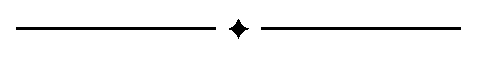
\includegraphics{diamondrule} is completely sufficient.
%%
\ifpdf%                                % if we use pdflatex
  \pdfoutput=1\relax                   % create PDFs from pdfLaTeX
  \pdfcompresslevel=9                  % PDF Compression
  \pdfoptionpdfminorversion=7          % create PDF 1.7
  \ExecuteOptions{pdftex}
  \usepackage{graphicx}                % allow us to embed graphics files
  \DeclareGraphicsExtensions{.pdf,.png,.jpg,.jpeg} % for pdflatex we expect .pdf, .png, or .jpg files
\else%                                 % else we use pure latex
  \ExecuteOptions{dvips}
  \usepackage{graphicx}                % allow us to embed graphics files
  \DeclareGraphicsExtensions{.eps}     % for pure latex we expect eps files
\fi%

%% it is recomended to use ``\autoref{sec:bla}'' instead of ``Fig.~\ref{sec:bla}''
\graphicspath{{figures/}{pictures/}{images/}{./}} % where to search for the images

\usepackage{microtype}                 % use micro-typography (slightly more compact, better to read)
\PassOptionsToPackage{warn}{textcomp}  % to address font issues with \textrightarrow
\usepackage{textcomp}                  % use better special symbols
\usepackage{mathptmx}                  % use matching math font
\usepackage{times}                     % we use Times as the main font
%\renewcommand*\ttdefault{txtt}         % a nicer typewriter font
\usepackage{cite}                      % needed to automatically sort the references
\usepackage{tabu}                      % only used for the table example
\usepackage{booktabs}                  % only used for the table example
%% We encourage the use of mathptmx for consistent usage of times font
%% throughout the proceedings. However, if you encounter conflicts
%% with other math-related packages, you may want to disable it.

%% In preprint mode you may define your own headline.
%\preprinttext{To appear in IEEE Transactions on Visualization and Computer Graphics.}

%% If you are submitting a paper to a conference for review with a double
%% blind reviewing process, please replace the value ``0'' below with your
%% OnlineID. Otherwise, you may safely leave it at ``0''.
\onlineid{0}

%% declare the category of your paper, only shown in review mode
\vgtccategory{Research}
%% please declare the paper type of your paper to help reviewers, only shown in review mode
%% choices:
%% * algorithm/technique
%% * application/design study
%% * evaluation
%% * system
%% * theory/model
\vgtcpapertype{proposal}

%% Paper title.
\title{Using Data Visualization to Pinpoint Mistakes in MIDI Practice Recordings}

%% This is how authors are specified in the journal style

%% indicate IEEE Member or Student Member in form indicated below
\author{Jeremy Grifski and Stephen Wu}
\authorfooter{
%% insert punctuation at end of each item
\item
 Jeremy Grifski is a student at The Ohio State University. E-mail: grifski.1@osu.edu.
\item
 Stephen Wu is a student at The Ohio State University. E-mail: wu.2719@osu.edu.
}

%other entries to be set up for journal
\shortauthortitle{Biv \MakeLowercase{\textit{et al.}}: Global Illumination for Fun and Profit}
%\shortauthortitle{Firstauthor \MakeLowercase{\textit{et al.}}: Paper Title}

%% Abstract section.
\abstract{
When a musician wants to practice their instrument, they often have to rely
on their peers or an instructor to help them isolate mistakes in their
technique. As an alternative solution, we are proposing a system to answer the
following question: how can we leverage data visualization to pinpoint mistakes
in music data? For the sake of scope, we have chosen to focus on MIDI recordings.
} % end of abstract

%% Keywords that describe your work. Will show as 'Index Terms' in journal
%% please capitalize first letter and insert punctuation after last keyword
\keywords{Music, Data Visualization, MIDI.}

%% ACM Computing Classification System (CCS).
%% See <http://www.acm.org/class/1998/> for details.
%% The ``\CCScat'' command takes four arguments.

\CCScatlist{ % not used in journal version
 \CCScat{K.6.1}{Management of Computing and Information Systems}%
{Project and People Management}{Life Cycle};
 \CCScat{K.7.m}{The Computing Profession}{Miscellaneous}{Ethics}
}

\vgtcinsertpkg

%%%%%%%%%%%%%%%%%%%%%%%%%%%%%%%%%%%%%%%%%%%%%%%%%%%%%%%%%%%%%%%%
%%%%%%%%%%%%%%%%%%%%%% START OF THE PAPER %%%%%%%%%%%%%%%%%%%%%%
%%%%%%%%%%%%%%%%%%%%%%%%%%%%%%%%%%%%%%%%%%%%%%%%%%%%%%%%%%%%%%%%%

\begin{document}

%% the only exception to this rule is the \firstsection command
\firstsection{Introduction}

\maketitle

Music is a profession and hobby enjoyed by many people. Unfortunately, the
field hasn't received a lot of attention from the technology community. To
this day, musicians still practice their instruments with little to no
benefit from technology.

One area of music that could really benefit from a technological upgrade would
be practice. After all, practice is usually something that occurs alone without
a lot of feedback. Without access to an instructor, musicians may find it difficult
to self-assess their abilities. They could all benefit from some sort of tool
to help pinpoint their mistakes.

In this project, we intend to build a data visualization dashboard which can
be used to compare practice MIDI files with professional MIDI files. The goal
is to isolate areas in the practice file which are most unlike the professional
file for the sake of improvement.

\section{Research Questions}

As mentioned previously, the major research question we will be looking to
address is the following: how can we leverage data visualization to pinpoint
mistakes in MIDI practice recordings?

Naturally, this question raises several underlying questions such as:

\begin{itemize}
\item What are practice areas and quantifiable data (pitch, tempo, etc.) that
we can gleam from MIDI recordings?
\item What are the most effective ways of visualizing those practice areas?
\item What are our options in analyzing MIDI files to visualize MIDI events
in a useful manner for musicians?
\item How useful is comparing MIDI recordings via velocity, sustain, and note
frequency over time graphs
\item Can we algorithmically generate useful automated feedback from analysis
of these MIDI recordings and graphs
\end{itemize}

In an effort to pinpoint mistakes, we will need to find the best ways to
represent our musical data, so the user will see value in the tool.

\section{Design Goals}

At a high level, we intend to construct a dashboard split into two panes: the
file pane and the graph pane.

The file pane will contain a list of active MIDI files which are each given a
color for encoding purposes. That means the dashboard will be able to support
about 20 simultaneous MIDI files due to the limits of color perception. This
should be more than enough considering the practicality of comparing that many
recordings.

Each file in the file pane will be able to be selected for viewing purposes
in the graph pane. When unselected, the file's background color will be neutral.
When selected, the file's background color will mirror its color in the graph
pane.

Meanwhile, the graph pane will contain several graphs:

\begin{itemize}
\item Notes versus Time (master graph)
\item Notes versus Frequency
\item Velocity versus Time
\item Sustain versus Time
\end{itemize}

As a stretch goal, each graph will be connected with the master graph for
filtering purposes. When a section of time is selected in the master graph,
all other graphs will be updated to reflect the new subsection of data. This
will allow a user to hone in on specific mistakes.

In addition, graphs will contain tooltips which will highlight areas with
the highest amount of mistakes. These tooltips will include high level notes
to assist the user in understanding the data.

Finally, the dashboard can be extended to include realtime recording and sheet
music comparison.

\section{Hardware and Software Requirements}

To complete this project, we require the following software:

\begin{itemize}
\item JavaScript: a web-based programming language
\item D3.js: a data visualization library
\item MIDI.js: a MIDI processing library
\item GarageBand: a MIDI editing tool
\item GitHub: a version control and project management tool
\item Travis CI: a continuous integration tool for testing
\end{itemize}

With this software, we should be able to build and test the entire system.

\section{Tasks and Metrics}

In order to verify the success of this project, we will be tracking several
tasks in GitHub. Namely, we will be designing and implementing the following:

\begin{itemize}
\item MIDI File Upload
\item MIDI File Pane
\item Notes versus Time Graph
\item Notes versus Frequency Graph
\item Velocity versus Time Graph
\item Sustain versus Time Graph
\item Mistake Analysis for Tooltips
\item Realtime Recording
\item Sheet Music Rendering and Comparison
\end{itemize}

Each of these tasks can probably be broken down into smaller tasks as they all
need to be designed, prototyped, and tested.

As for verifying that our design is good, we'll be testing it on musicians
of varying abilities. They will first play a song to generate a MIDI file,
then we will ask them to indicate any mistakes they felt they made. Finally,
we will compare their personal insight to the tool.

To take the research a step further, we would need to also gather insight from
professional reviewers to see how their thoughts vary from the results in the
tool.

\section{Initial Prototype}

\section{Evaluation}

Evaluation was done in two phases, an initial prototype on March 7, 2019 and an
updated prototype on April 6, 2019. Feedback was gathered from both phases to
evaluate and improve the product.

For the updated prototype evaluation, we shared the tool with one of our advisors.
Unfortunately, they hadn’t gotten around to the tool in time due to vis paper
deadlines. As a result, we decided to review the tool ourselves.

\subsection{Initial Prototype}

\subsection{Prototype Feedback}

In general, feedback was positive. However, there were a few things
that needed improvement in the original prototype. The following
list contains all feedback:

\begin{itemize}
  \item Colors
  \begin{itemize}
    \item Too closely related (light blue and dark blue)
    \item Yet, calming
  \end{itemize}
  \item Velocity plot
  \begin{itemize}
    \item Difficult to see differences in curves
    \item Plot may not be capturing appropriate data (summing velocities)
    \item Look into normalization
  \end{itemize}
  \item Target audience
  \begin{itemize}
    \item Musicians don't care about time steps - they want beats and measures
  \end{itemize}
  \item Interactivity
  \begin{itemize}
    \item Playback should animate graphs
  \end{itemize}
\end{itemize}

\subsection{Changes to Address Feedback}

To address some of the feedback from above, we decided to look into the
following changes:

\begin{itemize}
  \item Adding a time marker to show where we are in the song
  \item Changing velocity plot to be more expressive
  \item Reordering the color array so additional tracks have drastically different colors
  \item Add option for user to specify tempo, changing time to measure
\end{itemize}

So far, we’ve completed \#1 and \#2 for the updated prototype.

\subsection{Additional Feedback and Evaluation}

As an intermediate piano player, author Stephen’s thoughts on the tool were as follows:

\begin{itemize}
  \item Inherent limitations:
  \begin{itemize}
    \item Online, generated MIDI files are often lacking when compared to an actual song:
    \begin{itemize}
      \item Song may have a constant velocity for every note.
      \item Key signatures, tempo, and sustain may be missing.
    \end{itemize}
    \item Recorded MIDI files have some of these issues and more:
    \begin{itemize}
      \item Velocity is obtained, but this is not exactly reflective of playing on an acoustic piano, which is what would be typically used in performance. Keyboards, especially cheaper ones, are simply less expressive than acoustic pianos.
      \item If the user is off-time by even a beat, the whole song gets offset. If the user corrects their time and becomes on-time, this issue is resolved. This means the user needs to be playing to a metronome and correct any time lost, which adds additional requirements on their playing.
    \end{itemize}
    \item Preprocessing:
    \begin{itemize}
      \item Key signatures and tempo need to be manually added if needed for tool (it isn’t in the current stage).
      \item The MIDI file also needs to be edited to remove any wait in the beginning.
    \end{itemize}
  \end{itemize}
  \item Benefits:
  \begin{itemize}
    \item Where this tool thrives is helping identify insights that can’t be simply heard or seen in a recording.
    \item Users can upload and play their recordings.
    \item The velocity curve is probably the most novel item, since other tools (like GarageBand) provide the features of the Master Note graph.
    \being{itemize}
      \item Users can follow the sheet music and quickly see how they played different sections, e.g. if they played one forte section louder than another, or if they mistakenly played one forte section as piano.
    \end{itemize}
  \end{itemize}
\end{itemize}

\section{Conclusion}

It may seem odd to want to think of music in a visual way, but we feel our
system will have a positive impact on musicians who want to improve their
practice sessions.

\end{document}
